\documentclass[smaller,aspectratio=169]{beamer}
% This enables printing multiple pages on 1 pdf page (i.e. slide and notes)
\usepackage{pgfpages}

% Put notes on right side
\setbeameroption{show notes on second screen=right}
\mode<presentation>
{
  \usetheme[progressbar=frametitle]{metropolis}

  \setbeamercovered{transparent}
}

% this is to use British English conventions
\usepackage[british]{babel}
% this is to include images/plots/etc
\usepackage{graphicx}
\graphicspath{{figures/}}
% add movies
\usepackage{multimedia}
% this adds \footcite
\usepackage[backend=biber,style=authoryear,eprint=true, 
giveninits=true]{biblatex}
% this sets all maths fonts to the usual serif one
\usefonttheme[onlymath]{serif}
% this allows tikz graphics
\usepackage{tikz}
% externalize tikz to speed up compilation
%\usetikzlibrary{external}
%\tikzexternalize[prefix=cache/]
% this adds animations of tikz graphics (in suitable pdf viewers)
\usepackage[autoplay,loop,palindrome]{animate}
% this allows inclusion of standalone latex files
\usepackage{standalone}
% don't include appendix frames in numbering
\usepackage{appendixnumberbeamer}
% this allows more colours
\usepackage{xcolor}
\usepackage{amsmath}
\addbibresource{bibliography.bib}

\iffalse
    \bibliography{bibliography}
\fi

%Customise \footcite command
\DeclareCiteCommand{\footcite}[\mkbibfootnote]
  {\usebibmacro{prenote}}
  {\printnames[family-given][-3]{labelname}%
   \newunit
   \printfield{archivePrefix}
   \printfield{eprint}
   %\printfield{primaryClass}%
   \newunit
   \printlabeldateextra}
  {\addsemicolon\space}
  {\usebibmacro{postnote}}
  
\DeclareCiteCommand{\citea}
  {\usebibmacro{prenote}}
  {\printnames[family-given][-3]{labelname}%
   \newunit
   \printfield{archivePrefix}
   \printfield{eprint}
   %\printfield{primaryClass}%
   \newunit
   \printlabeldateextra}
  {\addsemicolon\space}
  {\usebibmacro{postnote}}

\makeatletter
\newlength\beamerleftmargin
\setlength\beamerleftmargin{\Gm@lmargin}
\makeatother
  
\newcommand{\rad}{\mathrm{rad}}
\newcommand{\tl}{\tilde{\ell}}
\newcommand{\tm}{\tilde{m}}
\newcommand{\rmd}{\mathrm{d}}

\title[Eccentric Kicks] % (optional, use only with long paper titles)
{Anomalies in the gravitational recoil of eccentric black-hole mergers with unequal mass ratios\footnote{arXiv:2101.11015\vspace{0.5 cm}}}

\author{
    \textbf{Miren~Radia}\textsuperscript{{1}} \and 
    Ulrich~Sperhake\textsuperscript{1} \and 
    Emanuele~Berti\textsuperscript{2} \and 
    Robin~Croft\textsuperscript{1}}

\institute
{
    \textsuperscript{1} Department of Applied Mathematics \& 
    Theoretical Physics, University of Cambridge\\
    \textsuperscript{2} Department of Physics \& Astronomy, 
    Johns Hopkins University
}

\date{DAMTP GR Seminar: 26 Feb 2021}
% - Either use conference name or its abbreviation.
% - Not really informative to the audience, more for people (including
%   yourself) who are reading the slides online

\subject{Numerical Relativity}
% This is only inserted into the PDF information catalog. Can be left
% out.

% Uncomment \logo and comment \titlegraphic to put University logo on every page
%\logo{\includegraphics[height=0.5cm]{uni-cam-logo}\hspace{1 cm}}
\titlegraphic{
    \vspace{6 cm}
    \includegraphics[width=2cm]{grchombo-logo.png}
    \hfill
    \includegraphics[width=3cm]{uni-cam-logo.eps}
%     \vspace{-2 cm}
    }
% 
% 
% Delete this, if you do not want the table of contents to pop up at
% the beginning of each subsection:
% \AtBeginSubsection[]
% {
%   \begin{frame}<beamer>{Outline}
%     \tableofcontents[currentsection,currentsubsection]
%   \end{frame}
% }


% If you wish to uncover everything in a step-wise fashion, uncomment
% the following command: 

% \beamerdefaultoverlayspecification{<+->}


\begin{document}

\begin{frame}
  \titlepage
%   \vspace{2 cm}
    %\note[item]{Thank organisers}
\end{frame}

\note
{   
    \begin{itemize}
        \item<.-> 
            Thank the organisers for invitation.
        \item<.-> 
            Sorry for there not being pizza. I hope this doesn't affect
            your opinion of my talk.
        \item<.-> 
            Mention other collaborators.
        \item<.-> 
            Say this was recently put on the arXiv.
    \end{itemize}
}


\begin{frame}{Outline}
  \tableofcontents
  % You might wish to add the option [pausesections]
\end{frame}


% Structuring a talk is a difficult task and the following structure
% may not be suitable. Here are some rules that apply for this
% solution: 

% - Exactly two or three sections (other than the summary).
% - At *most* three subsections per section.
% - Talk about 30s to 2min per frame. So there should be between about
%   15 and 30 frames, all told.

% - A conference audience is likely to know very little of what you
%   are going to talk about. So *simplify*!
% - In a 20min talk, getting the main ideas across is hard
%   enough. Leave out details, even if it means being less precise than
%   you think necessary.
% - If you omit details that are vital to the proof/implementation,
%   just say so once. Everybody will be happy with that.

\section{Introduction}

\begin{frame}{What are kicks?}
    \begin{itemize}
        \item<+-> 
            \alert{Asymmetric} emission of GWs will carry a net linear 
            momentum.
        \note[item]<.->{
            It has been known for a long time that GWs carry energy and
            angular momentum.}
        \note[item]<.->{
            The carrying of linear momentum has been known for slightly
            less time .}
        \item<+->
            Conservation of momentum means a recoil (or \alert{kick}) 
            is imparted to the emitting 
            system\footcite{Bonnor1961-wy,Peres:1962zz,Bekenstein:1973zz}.
        \item<+->
            For binary BH mergers, the necessary \alert{asymmetry} can be 
            e.g. unequal masses or misaligned spins.
        \note[item]<.->{
            An equal-mass non-spinning black-hole binary cannot emit a
            net linear momentum by symmetry.}
        \item<+->
            Astrophysical consequences: compare kick velocity $v$ with escape 
            velocity $v_{\text{esc}}$ of various astrophysical environments
            \begin{itemize}
                \item<.->
                    Globular clusters: 
                    $v_{\text{esc}}=\mathcal{O}(10\text{ km/s})$,
                    quasicircular non-spinning BBH mergers: 
                    $v = \mathcal{O}(100\text{ km/s})$.
                \item<.->
                    Can use kicks to constrain growth theories of 
                    SMBHs at the centre of dark matter halos.
            \end{itemize}
        \note[item]<.->{
            We can also use kicks to estimate the rate of second
            generation mergers between black-holes that have already
            formed from mergers.}
        \item<+->
            The study of recoiling GW emitters may help us understand
            astrophysical sources better.
        \note[item]<.->{
            A recoiling postmerger BH can induce
            a blue (or red) shift on parts of its GW signal that
            may be exploited in future GW observations to directly
            measure kicks.}
        \note[item]<.->{
            The effect of kicks should be taken into account in future
            ringdown tests of GR with 3G GW detectors to avoid systematic
            biases.}
    \end{itemize}
\end{frame}

\begin{frame}{Why consider eccentricity?}
    \begin{itemize}
        \item<+-> 
            We still don't know how BH binaries form 
            (there are several suggested \alert{formation channels})!
        \note[item]<.->{
            Currently it is widely believed that most BH binaries formed
            from primordial star binaries in isolated systems.}
        \note[item]<.->{
            However there are several recent studies which suggest the 
            proportion of BH binaries formed dynamically are much higher
            than what was previously thought.}
        \item<+->
            For \alert{isolated binary} systems, GW emission acts to 
            circularize orbits.
        \item<+->
            Orbital Eccentricity expected to be a distinguishing feature of 
            \alert{dynamical} formation channels in e.g. globular 
            clusters, galactic nuclei, etc.
        \note[item]<.->{
            Eccentricity can be used as a means to determine formation
            channels of BH binaries.}
        \item<+->
            No evidence from LIGO O1 and O2 runs\footcite{Salemi:2019owp} 
            but GW190521 is potentially consistent with\footcite{Gayathri:2020coq} 
            $e\simeq0.7$.
        \item<+->
            Also just another way to possibly \alert{accentuate} asymmetry.
        \note[item]<.->{
            Since kicks are caused by asymmetry, eccentricity is a natural
            ingredient to add in order to enhance/modify the kick.}
    \end{itemize}
\end{frame}

\section{Setup and Methods}

\subsection{Brief recap of Numerical Relativity methods}
\begin{frame}{The 3+1 formalism}
    \begin{columns}
        \begin{column}{0.6\columnwidth}
            \small
            \begin{itemize}
                \note[item]<.->{ 
                    I will go through this quickly as I assume most people here 
                    will have seen this before.}
                \item<+->
                    Foliate spacetime by spatial hypersurfaces $\Sigma_t$ 
                    indexed by a global time function $t$.
                \item<+->
                    Choose \alert{adapted} coordinates $(t,x^i)$, where the 
                    metric takes the form
                    \begin{equation*}
                        ds^2 =  -\alpha^2\,\rmd t^2 + \gamma_{ij}\left(
                            \rmd x^i + \beta^i\, \rmd t\right)\left(\rmd x^j + 
                            \beta^j\, \rmd t\right), 
                    \end{equation*}
                    where $\alpha$ is the \alert{lapse}, $\beta^i$ is the 
                    \alert{shift}, and $\gamma_{ij}$ is the 
                    \alert{spatial metric}.
                \note[item]<.->{
                    The lapse and shift are our gauge variables that determines 
                    how our coordinates behave.}
                \item<+->
                    Introduce the \alert{extrinsic curvature}, given by
                    \begin{equation*}
                        K_{ij} = -\frac{1}{2}(\mathcal{L}_n\gamma)_{ij}.
                    \end{equation*}
                \note[item]<.->{
                    Note the sign convention of the extrinsic curvature which 
                    is standard in numerical relativity (but differs to other 
                    conventions).}
                \item<+->
                    Projecting the Einstein equation yields the 
                    \alert{ADM evolution and constraint} eqautions.
                \item<+->
                    Only \alert{weakly} hyperbolic so not suited for numerical 
                    evolution.
                \note[item]<.->{
                    Need strong hyperbolicity for a well-posed IVP in order to 
                    evolve stably although this is not sufficient.}
            \end{itemize}
        \end{column}
        \begin{column}{0.4\columnwidth}
            \resizebox{\columnwidth}{!}
            {
                \centering
                \begin{tikzpicture}[scale=1.2]
                    %top surface
                    \draw (-2,1) to[out=15,in=-165] (2,1);
                    \draw (-1.6,1.4) to[out=15,in=-165] (2.4,1.4);
                    \draw (-1.6,1.4) to (-2,1);
                    \draw (2.4,1.4) to (2,1);
                    \node at (-2.5, 1.2) {$\Sigma_{t+\delta t}$};
                    
                    % bottom surface
                    \draw (-2,-1) to[out=15,in=-165] (2,-1);
                    \draw (-1.6,-0.6) to[out=15,in=-165] (2.4,-0.6);
                    \draw (-2,-1) to (-1.6,-0.6);
                    \draw (2,-1) to (2.4,-0.6);
                    \node at (-2.5, -0.8) {$\Sigma_t$};
                    
                    %normal arrow
                    \draw[thick] (-0.5,-0.7) to (-0.5,1.07);
                    \draw[dotted, thick] (-0.5,1.07) to (-0.5,1.27); 
                    \draw[thick,-latex] (-0.5,1.27) to (-0.5,1.8) 
                        node [above] {$n^\mu = \alpha(\rmd t)^\mu$};
                    
                    %time arrow
                    \draw[thick] (-0.5,-0.7) to (0.5,0.93);
                    \draw[dotted,thick] (0.5,0.93) to (0.623,1.13);
                    \draw[thick,-latex] (0.623,1.13) to (0.954,1.67);
                    \node at (1.8,1.67) [above] 
                        {$t^\mu = \alpha n^\mu + \beta^\mu$};
                    
                    %beta arrow
                    \draw[-latex] (-0.5,1.27) to (0.623,1.13);
                    \node at (0,1.2) [above] {$\beta^i$};
                    
                    %point on bottom surface
                    \draw[fill=red] (-0.5,-0.7) circle (0.05);
                    \node at (-0.5,-1.2) {$(t,x^i)$};
                    
                    %point on top surface
                    \draw[fill=red] (0.623,1.13) circle (0.05);
                    \node at (1.35,0.7) {$(t+\delta t,x^i)$};
                    
                    %normal point on top surface
                    \draw[fill=red] (-0.5,1.27) circle (0.05);
                    \node at (-2.2,1.7) 
                    {$(t+\delta t, x^i - \beta^i \delta t)$};
                \end{tikzpicture}
            }
        \end{column}
    \end{columns}
\end{frame}

\begin{frame}{Towards suitable formulations of the Einstein equations}
    \begin{itemize}
    \small
    \item<+->
        Introduce a \alert{conformal} decomposition of the metric and decompose 
        the extrinsic curvature:
        \begin{equation*}
            \gamma_{ij} = \frac{1}{\chi}\tilde{\gamma}_{ij},\qquad K_{ij} =
            \frac{1}{\chi}\left(\tilde{A}_{ij} + 
            \frac{1}{3}K\tilde{\gamma}_{ij}\right),
        \end{equation*}
        where $\chi = (\det \gamma)^{-1/3}$.
    \note[item]<.->{ 
        The choice of this conformal factor allows the $\chi$ to smoothly go to 
        0 when the physical metric elements blow up and the conformal metric
        remains well-behaved.}
    \item<+->
        Introduce the \alert{conformal connection functions}: 
        $\tilde{\Gamma}^i=\tilde{\gamma}^{jk}\tilde{\Gamma}^i_{jk}$.
    \note[item]<.->{
        The introduction of the conformal connection functions is key to 
        removing terms that spoil strong hyperbolicity.}
    \item<+->
        This is the basis of commonly used strongly hyperbolic formulations in 
        NR, in particular the ones we use: BSSNOK\footcite{Nakamura:1987zz,
        Shibata:1995we,Baumgarte:1998te} and CCZ4\footcite{Alic:2011gg}.
    \note[item]<.->{
        In the BSSNOK formulation, the evolution equations are modified using 
        the constraint equations.}
    \note[item]<.->{
        In the CCZ4 formulation, an extra 4-vector is introduced which vanishes
        on the constraint hypersurface in its solution space.}
    \item<+->
        Also very important to pick a gauge which is strongly 
        singularity avoiding and can stably evolve moving BHs. We use the 
        moving puncture 
        gauge\footcite{Baker:2005vv,Campanelli:2005dd,Alcubierre:2002kk,
        Bona:1994dr}, which has proved remarkably robust at evolving BHs over 
        the past 15 years or so.
    \note[item]<.->{
        It is still not understood rigorously why the moving puncture 
        gauge works so well whereas other gauges which also give a strongly 
        hyperbolic system fail. There are only heuristic arguments. If anyone 
        proves this, please let me know!}
    \end{itemize}
    \vspace{0.5 em}
\end{frame}

\begin{frame}{Extraction of Gravitational Waves in Numerical Relativity}
    \begin{itemize}
    \item<+->
        We use the complex \alert{Weyl scalar} $\Psi_4$ to extract 
        gravitational waves. It is given by
        \begin{equation}
            \Psi_4 = C_{\alpha\beta\gamma\delta}k^\alpha \bar{m}^\beta k^\gamma 
            \bar{m}^\delta,
        \end{equation}
        where $C_{\alpha\beta\gamma\delta}$ is the Weyl tensor and 
        $\left\{l^\mu,k^\mu,m^\mu,\bar{m}^\mu\right\}$ is the complex null 
        tetrad in the \alert{Newman-Penrose formalism} 
        where the spacetime metric can be written as
        \begin{equation}
            g_{\mu\nu} = -l_\mu k_\nu -k_\mu l_\nu + m_\mu \bar{m}_\nu + 
            \bar{m}_\mu m_\nu.
        \end{equation}
    \note[item]<.->{
        In NR, finding this null tetrad is nontrivial but we use an 
        approximation known as the Kinnersley tetrad.}
    \item<+->
        In the \alert{linearized approximation}, for a plane wave in TT gauge, 
        we find
        \begin{equation}
        \Psi_4 = \ddot{h}^+-\mathrm{i}\ddot{h}^\times,
        \end{equation}
        where $h^+$ and $h^\times$ are the two polarization amplitudes.
    \note[item]<.->{
        Hopefully plane waves in the linearized approximation and TT gauge
        are all familar concepts from undergraduate/graduate GR courses.}
    \item<+->
        We typically extract the values of $\Psi_4$ on multiple spheres at 
        fixed finite coordinate radius. We can then extrapolate to null 
        infinity assuming the asymptotic falloff
        \begin{equation}
            \Psi_4 \sim \frac{1}{r} + \mathcal{O}\left(\frac{1}{r^2}\right).
        \end{equation}
    \note[item]<.->{
        This assumption is the peeling property which Leonhard talked about
        earlier in this seminar series.}
    \end{itemize}
\end{frame}


\subsection{BH binary configurations}

\begin{frame}{BH binary configurations}
	\begin{center}
    \movie[
        width=0.7\textwidth,
        height=0.205\textwidth,
        poster
        ]
        {
            \includegraphics[width=0.7\textwidth]
            {bh-schematic-animated-0.png}
        }
        {./figures/bh-schematic-animated.mp4}
    \end{center}

    \begin{itemize}
        \item<1->
            We consider \alert{four sequences} (\texttt{sq2:3}, \texttt{sq1:2}, 
            \texttt{lq1:2} and \texttt{sq1:3}) with \alert{three different 
            mass ratios}: $q=2/3$, $1/2$ and $1/3$\footnote{
            Maximum kick in quasicircular case occurs at $q\simeq1/2.77$.}.
        \note[item]<1->{\footnotesize
            We chose the mass ratios to cover the interesting part of the 
            plot of quasicircular kick velocity against mass ratio 
            (will compare with this later).}
        \note[item]<1->{\footnotesize
            A sequence is constructed by first finding the tangential momentum
            that gives a quasicircular configuration (using a PN formula) given
            specified initial coordinate separation and masses. Then the 
            tangential momentum is progressively reduced whilst holding the 
            binding energy constant. This means the initial separation, $D$
            increases. For each sequence, we conduct around 60-80 simulations.}
        \note[item]<1->{\footnotesize
            Somewhat arbitrary choice to keep the binding energy constant
            (rather than e.g. the initial separation) but this at least ensures
            the inspiral phase duration within a sequence is comparable.}
        \item<2->
            Two sequences for $q=1/2$, one longer\footnote{In the 
            quasicircular limit: short sequence configurations do $\sim3$ 
            orbits and long $\sim6$ orbits} to identify any 
            possible artifacts due to short inspiral phases.
        \item<3->
            No well-defined notion of eccentricity in full GR, 
            so we use an estimate coming from 
            PN theory\footcite{Memmesheimer:2004cv}: 
            $e_t$ (in harmonic coordinates).
        \note[item]<3->{\footnotesize
            In this PN formalism, there are 3 eccentricity parameters which 
            are related to one another. The choice of which one to use is 
            arbitrary and they give comparable results. In the Newtonian limit,
            they reduce to the usual Keplerian eccentricity parameter.}
        \note[item]<3->{\footnotesize
            The eccentricity estimate should be taken with a pinch of salt as
            the inspiral phase of the simulations (even the long sequence) is 
            relatively short. Nevertheless, it provides us with a means
            to quantify the deviations from quasicircularity.}
    \end{itemize}
	\vskip 0.5em
\end{frame}

\subsection{Numerical implementation}

\begin{frame}{Numerical implementation}
    \small
    \begin{itemize}
        \item<+->
            \textsc{GRChombo}\footcite{Clough:2015sqa} was used with 
            \alert{CCZ4} for \texttt{sq2:3} and \texttt{sq1:3}.
        \note[item]<.->{\scriptsize
            GRChombo was developed a few years ago here in the GR group with 
            collaborators from KCL and QMUL. I am a current developer of the 
            code}
        \note[item]<.->{\scriptsize
            I believe this is the first time GRChombo has been used in a study
            involving conventional BBHs. It was mainly intended for more exotic
            spacetimes}
        \item<+->
            \textsc{Lean}\footcite{Sperhake:2006cy} was used with 
            \alert{BSSNOK} for \texttt{sq1:2} and \texttt{lq1:2}.
        \note[item]<.->{\scriptsize
            Lean is Uli's code which has been around since the mid-2000s. It has
            been used many times for BBH simulations.}
        \item<+->
            Both codes use the method of \alert{finite differences} where the
            continuum is approximated by a discrete number of points.
            The \alert{method of lines} is used for evolution with fourth order 
            time integration and sixth order spatial discretization.
        \note[item]<.->{\scriptsize
            Finite differencing is probably the canonical way of solving
            PDEs using computers but there are of course other methods.}
        \note[item]<.->{\scriptsize
            In the method of lines, the spatial discretization is made
            independent to the time stepping. This allows us to use standard
            ODE integration methods for the time integration, in particular 
            RK4.}
        \item<+->
            Both codes use Berger-Oliger style \alert{mesh refinement} where 
            the grid consists of a hierarchy of meshes with increasing 
            resolution in order to suitably resolve the BHs.
        \note[item]<.->{\scriptsize
            Mesh refinement is used to reduce computational expense. It would be
            prohibitively expensive to use the same resolution everywhere
            in the computational domain.}
        \begin{itemize}
            \item<.-> 
                \textsc{Lean} uses the tried and tested method of 
                \alert{moving boxes} based mesh refinement.
            \note[item]<.->{\scriptsize
                The method of moving boxes has been used for well over a decade 
                for BBH simulations.}
            \item<.->
                \textsc{GRChombo} uses a more \alert{adaptive} mesh refinement 
                that allows a wider variety of mesh structures.
            \note[item]<.->{\scriptsize
                Fully adaptive mesh refinement codes have not been widely used
                for BBH simulations so as part of this project we compared
                the results of oour code in order to ensure we were getting
                consistent results.}
        \end{itemize}
        \item<+->
            Both codes used the \textsc{TwoPunctures}\footcite{Ansorg:2004ds} 
            spectral solver for \alert{Bowen-York 
            puncture}\footcite{Bowen:1980yu} initial data
        \note[item]<.->{\scriptsize
            Bowen-York data is a conformally flat solution of the constraints 
            for multiple
            boosted, spinning BHs. It is not exactly the Kerr solution (in the 
            case of 1 BH) - there don't exist conformally flat coordinates 
            for Kerr so includes some extra stuff which we call the junk 
            radiation.}
    \end{itemize}
    \vspace{0.5 em}
\end{frame}

\subsection{Diagnostic quantities}
\begin{frame}{Diagnostic quantities}
	\begin{itemize}
		\item<+->
			Radiated energy $E^{\rad}$, 
			linear momentum $\mathbf{P}^{\rad}$ and 
			angular momentum $\mathbf{J}^{\rad}$ computed \alert{directly} 
			from extracted $\Psi_4$ values on extraction spheres e.g.
			\begin{equation}
				\mathbf{P}^{\rad}(t) = \lim_{r\to\infty}\frac{r^2}{16\pi}
				\int_{t_0}^t\rmd t^\prime\oint_{S^2_r}\rmd\Omega\,
				\hat{\mathbf{e}}_r\left|\int_{-\infty}^{t^\prime}\rmd t^{\prime\prime}\,
				\Psi_4\right|^2.
				\label{eq:Prad}
			\end{equation}
        \note[item]<.->{
            Given we were using a finite computational domain, we extracted 
            $\Psi_4$ at finite radii and then for several configurations
            extrapolated our results to null infinity in order to obtain an
            error estimate.}
        \note[item]<.->{
            The integration limit $t_0$ is chosen to exclude the contribution
            of the junk radiation.}
		\item<+->
			Kick obtained from $\mathbf{v}=-\mathbf{P}^{\rad}/M_{\text{fin}}$.
        \note[item]<.->{
            Kicks are much smaller than the speed of light so can ignore
            relativistic effects here.}
        \note[item]<.->{
            The final mass of the post-merger BH is computed using the 
            difference between the initial ADM mass and the radiated energy. The 
            final spin is computed similarly.}
		\item<+->
			Also computed\footnote{By symmetry $P^\rad_z=0$.} 
			$\mathbf{P}^{\rad}$
			from multipolar amplitudes of $\Psi_4=\sum_{\ell,m}\psi_{\ell,m}\left[{}_{-2}Y^{\ell,m}\right]$:
			\begin{multline}
				P_+(t) = P^\rad_x(t) + \mathrm{i}P^\rad_y(t)
				 = \lim_{r\to\infty}\frac{r^2}{8\pi}\sum_{\tl=2}^{\infty}
				 \sum_{\tm=-\tl}^{\tl}\int_{t_0}^t\rmd t^{\prime}
				\left\{\left(\int^{t^\prime}_{-\infty}\rmd t^{\prime\prime}\, 
				\psi_{\tl,\tm}\right)\right.\\
				\left.\times\left(\int_{-\infty}^{t^\prime} 
				\left[a_{\tl,\tm}\bar{\psi}_{\tl,\tm+1}+ 
				b_{\tl,-\tm}\bar{\psi}_{\tl-1,\tm+1}-
				b_{\tl+1,\tm+1}\bar{\psi}_{\tl+1,\tm+1}\right]
				\rmd t^{\prime\prime}\right)\right\},
				\label{eq:P+rad}
			\end{multline}
        \note[item]<.->{
            The details of this formula are unimportant but what should be noted
            is that the contribution to each $\tilde{\ell}$ and $\tilde{m}$ 
            term in the sum involves an overlap between several different modes
            of $\Psi_4$.}
			\vspace{0.5 em}
	\end{itemize}

\end{frame}

\section{Results}

{
\setbeamercolor{background canvas}{bg=black}
\begin{frame}{Visualisation}
    %\vspace{-1 em}
    %\hspace*{-11 mm}%
	\begin{center}
    \movie[
        width=\textwidth,
        %height = 0.47\textwidth,
        poster
        ]
        {
           \includegraphics[width=\textwidth]{eckick-q3-p0.085-0000.png} 
        }
        {./figures/eckick-q3-p0.085-spedup3.mp4}
    \end{center}
    \note[item]<.->{
        Point out that the kick has been sped up at the end because it's very
        slow in simulation time.}
\end{frame}
}

\subsection{Recoil velocity, radiated energy and final spin}

\begin{frame}{Recoil velocity, radiated energy and final spin}
    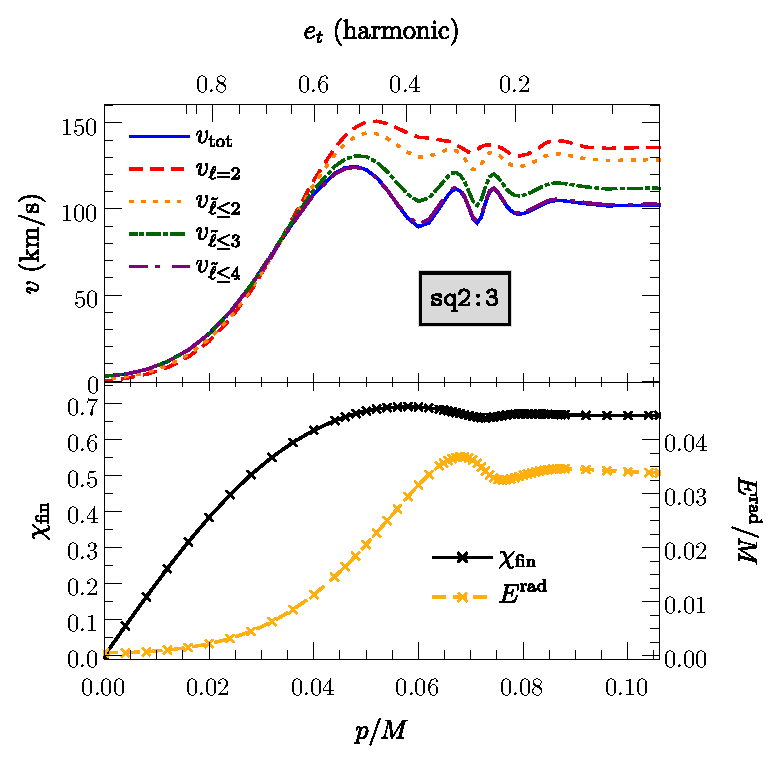
\includegraphics[width=0.45\linewidth]{kick-q1.5-wlabel.eps}
    \hfill
    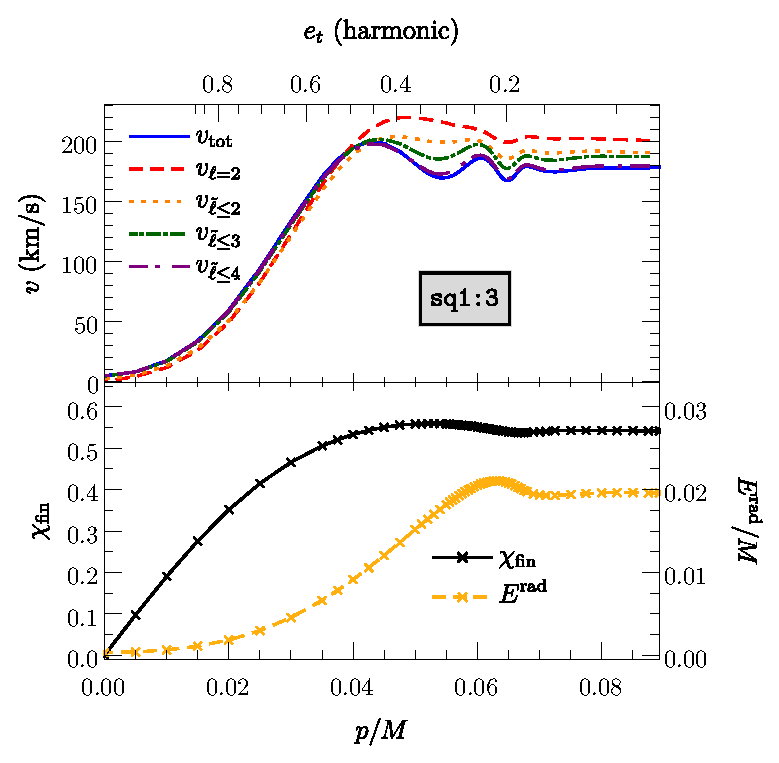
\includegraphics[width=0.45\linewidth]{kick-q3-wlabel.eps}
    \note[item]<.->{
        This slide is our main plot for the \texttt{sq2:3} and \texttt{sq1:3}
        sequences.}
    \note[item]<.->{
        In the top panel we have plotted the kick velocity in km/s as a 
        function of initial tangential momentum $p$. This is the blue solid 
line.}
    \note[item]<.->{
        We have also plotted the contribution from different partial sums
        in Eq.~\eqref{eq:P+rad}. The red dashed line is the contribution
        from $\ell=2$ modes of $\Psi_4$ only.}
    \note[item]<.->{
        The PN eccentricity estimate is also shown at the top. Note that it is
        nonlinear.}
    \note[item]<.->{
        In the bottom panel, we have plotted the radiated energy and final spin
        of the post-merger BH.}
    \note[item]<.->{
        Each cross corresponds to an in individual simulation.}
\end{frame}

\begin{frame}{Recoil velocity, radiated energy and final spin}
	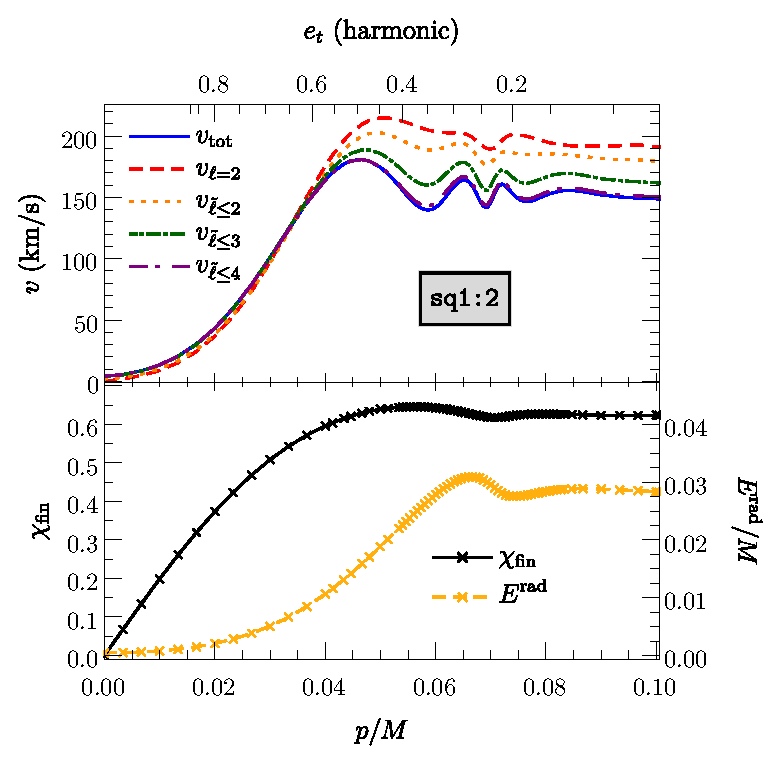
\includegraphics[width=0.45\linewidth]{kick-q2-wlabel.eps}
	\hfill
	\includegraphics[width=0.45\linewidth]{kick-q2l-wlabel.eps}
	\note[item]<.->{
        The slide is the same as the previous but for the \texttt{sq1:2} and
        \texttt{lq1:2} sequences (so both mass ratio $q=1/2$).}
    \note[item]<.->{
        Our first result is that the kick is maximised for moderate 
        eccentricities $e_t\approx 0.5$. For \texttt{sq2:3}, \texttt{sq1:2} and
        \texttt{lq1:2}, the amplification is about 25\% about the same as
        for the superkicks. For \texttt{sq1:3} it is about 12\%.
        We also get a slightly smaller kick (compared to the quasicircular 
        value) for lower but nonzero eccentricities.}
    \note[item]<.->{
        Our next observation is an oscillatory pattern in the kick velocity as 
        a function of $p$ or eccentricity. These oscillations seem to differ
        in their location to that of the radiated energy and final spin.
        The long sequence was added to check whether these oscillations were
        due to the short inspiral but remarkably the oscillations are more
        pronounced here.}
    \note[item]<.->{
        Considering the various truncations of the radiated momentum sum we see
        that the oscillations are present at every level (even quadrupole
        contributions only) but the effect is somewhat milder.}
    \note[item]<.->{
        Increasing the number of terms in the partial sums seems to 
        systematically decrease the kick.}
\end{frame}

\begin{frame}{Observations}
	\begin{columns}
		\column{0.4\textwidth}
			\centering
			\only<.->{
				\includegraphics[width=\columnwidth]{kick-q2l-wlabel.eps}
			}
		\column{0.6\textwidth}
			\begin{itemize}
                \note[item]<.->{
                    This slide is just summarizing what I have already said.}
				\item<.-> 
					\alert{Maximum} kick occurs at $e\sim0.5$ and 
					is about 22/22/25/12\% larger than the 
					quasicircular value for 
					\texttt{sq2:3}/\texttt{sq1:2}/\texttt{lq1:2}/\texttt{sq1:3}.
				\item<+->
					\alert{Oscillatory} behaviour in $v=v(p)$ 
					which increases in 
					frequency and amplitude for longer inspirals. 
					If this pattern continues,
					we would expect the kick to depend 
					\alert{highly sensitively} for even longer inspirals
                \note[item]<.->{
                    I preface this statement with ``if'' because extrapolating
                    based on two data points is not usually the most reliable
                    method.}
				\item<+->
					Fewer/less pronounced oscillations in radiated 
					energy/final spin with different extrema.
				\item<+->
					Oscillations present in all considered partial 
					sums of Eq.~\eqref{eq:P+rad},
					albeit somewhat less pronounced.
				\item<+->
					Higher-order terms with $\tl>2$ \alert{decrease} the kick.
			\end{itemize}
	\end{columns}
\end{frame}

\begin{frame}{Comparison with quasicircular kicks}
    \begin{columns}
        \begin{column}{0.5\textwidth}
            \begin{itemize}
                \item<+->
                    This figure shows the \alert{range} of recoil velocities 
                    obtained
                    for each sequence.
                \note[item]<.->{
                    The short sequences are in gold and the long sequence is
                    in red.}
                \item<.->
                    The blue line is a \alert{functional fit}\footnotemark~  
                    of kick velocity against the symmetric mass ratio $\eta$ in 
                    the \alert{quasicircular} case.
                \note[item]<.->{
                    Note that we have covered around the interval containing the
                    maximum kick in the quasicircular case.}
                \item<.->
                    We exclude the plunge limit (i.e. those configurations with
                    $p<p_{\max}$).
                \note[item]<.->{
                    Otherwise the range would go to almost zero. We are
                    interested in the oscillating regime.}
            \end{itemize}
        \end{column}
        \begin{column}{0.5\textwidth}
            \centering
            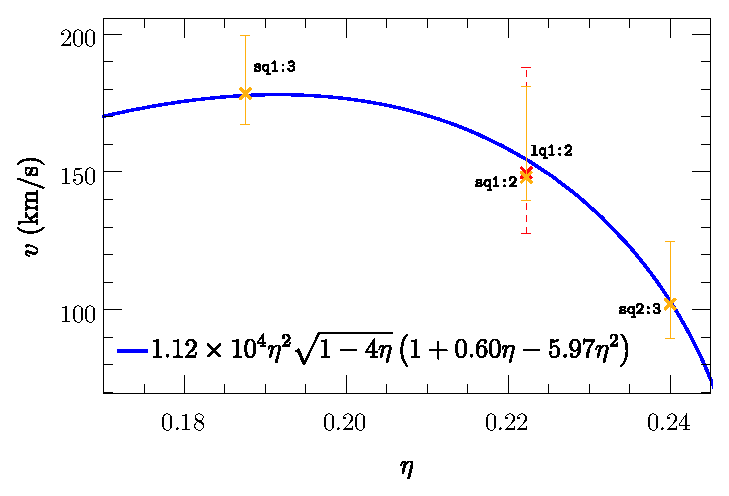
\includegraphics[width=\columnwidth]{quasicircular-fit2.eps}
        \end{column}
    \end{columns}
    \footnotetext{\citea{Healy:2017mvh}}
\end{frame}


\subsection{Kick angle}
\begin{frame}{Kick angle}
	\begin{columns}
		\column{0.6\textwidth}
			\begin{itemize}
                \note[item]<1->{
                    We now try to understand the origin of the oscillations.}
				\item<1->
					Only ``special'' direction is the \alert{apoapsis}.
                \note[item]<1->{
                    The apoapsis is the axis along which the separation of the
                    two objects is greatest in the Kepler problem. You may be
                    familiar with the term aphelion which is specific to the 
                    sun.}
                \note[item]<1->{
                    In the superkick case, the orientation of the spin
                    is picked out and there is a known sinusoidal dependence
                    of the kick on the angle of the spin in the orbital plane}
				\item<2->
					Want to look at \alert{infall direction} 
					relative to apoapsis.
				\item<3-> 
					No good definition of infall direction so 
					use \alert{kick angle}:
					\begin{equation}
					\vartheta = \text{arg}(v_x + \mathrm{i}v_y).
					\end{equation}
                \note[item]<3->{
                    If we interpret the gravitational recoil to be predominantly
                    generated by the excess beaming of GWs in the direction of 
                    the smaller and faster BH during the merger phase, this 
                    angle can serve as an approximation to the infall 
                    direction.}
			\end{itemize}
			\centering
			\only<-2>{\vspace{0.5\textheight}}
			\only<3->{
			\resizebox{!}{0.5\textheight}
			{
				%\tikzexternaldisable
				\begin{tikzpicture}
					% line connecting BHs
					\draw[dashed] (-3.46410161514,-2) -- (1.73205080757,1);
					
					% small BH
					\filldraw[fill = black] (-3.46410161514,-2) circle (0.3);
					\draw[very thick,-latex] (-3.46410161514,-2) -- 
					(-2.71410161514,-3.29903810568);
					\node[anchor=west] at (-2.71410161514,-3.29903810568) {$\mathbf{v}_1$};
					\node[color=white] at (-3.46410161514,-2)  {$M_1$};
					\foreach \r in {2,2.2,2.4,2.6,2.8,3,3.2}
					\draw[domain=-70:-50,smooth] plot 
					({-3.46410161514 + \r*cos(\x)},{-2+\r*sin(\x)});
					
					% big BH
					\filldraw[fill = black] (1.73205080757,1) circle (0.6);
					\draw[very thick,-latex] (1.73205080757,1) -- 
					(1.13205080757,2.03923048454);
					\node[anchor=east] at (1.13205080757,2.03923048454) {$\mathbf{v}_2$};
					\node[color=white] at (1.73205080757,1) {$M_2$};
					\foreach \r in {2,2.4,2.8}
					\draw[domain=140:100] plot 
					({1.73205080757+ \r*cos(\x)},{1+\r*sin(\x)});
					
					% centre of mass
					\draw[very thick,-latex] (0,0) -- (0.5,-0.86602540378);
					\node[anchor=north west] at (0.5,-0.86602540378) 
					{$\mathbf{P}^{\mathrm{rad}}$};
					\draw[very thick,-latex] (0,0) -- (-0.5,0.86602540378);
					\node[anchor=south east] at (-0.5,0.86602540378) {$\text{recoil}$};
					
					\filldraw[color=white, fill=red] (0,0) circle (0.1);
					
					\node at (3,-3) {Reproduced from \cite{Wiseman:1992dv}};
				\end{tikzpicture}
				%\tikzexternalenable
		}
		}
		\column{0.4\textwidth}
			\only<-3>{
				\vphantom{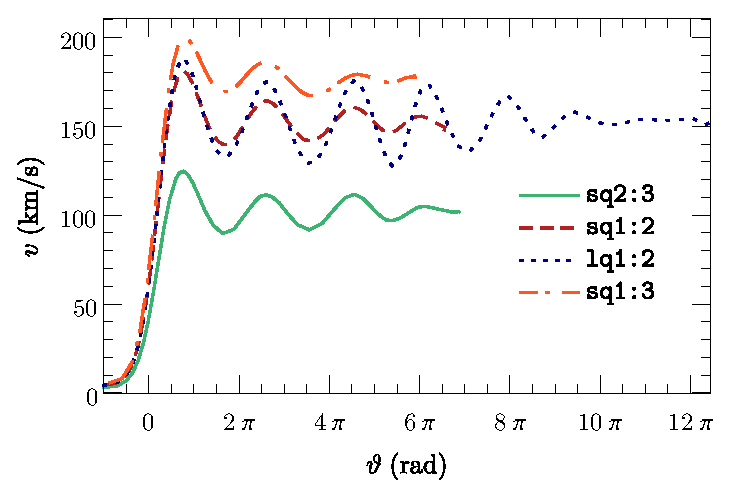
\includegraphics[width=\columnwidth]{kick-theta.eps}}
			}
			\only<4->{
				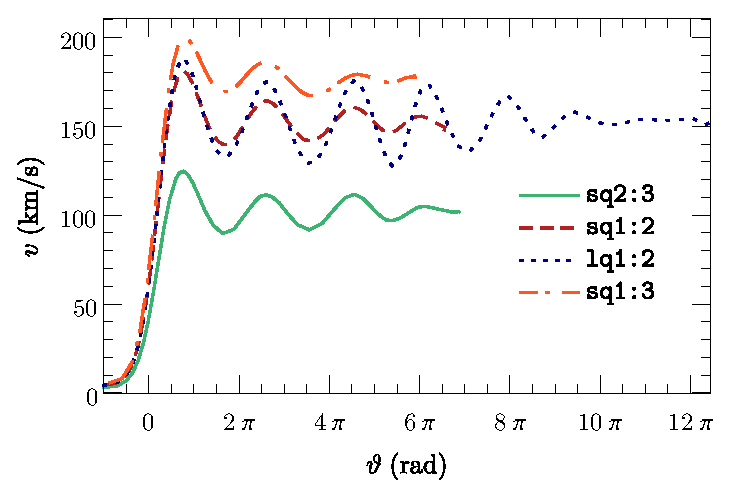
\includegraphics[width=\columnwidth]{kick-theta.eps}
			}
			\note[item]<4->{
                This figure shows the kick velocity plotted against the angle
                $\vartheta$ where we have added $2n\pi$ to ensure $\vartheta$
                is monotonic as a function of the initial tangential momentum 
                $p$.}
			\vspace{-2 em}
			\begin{itemize}
				\item<4->
					Naively might expect $2\pi$ periodicity...
                \note[item]<4->{
                    Here the oscillations have an almost constant frequency
                    which is not really dependent on the mass ratio.}
				\item<5->
					...but we mustn't forget \alert{apsidal precession} 
					(cf. Mercury) which we would expect to 
					slightly decrease the period.
                \note[item]<5->{
                    Recall the perihelion precession of Mercury which you will
                    have learnt about as an undergraduate. We believe this is
                    the cause of deviation from $2\pi$ periodicity.}
			\end{itemize}
	\end{columns}
\end{frame}

\subsection{Waveform observations}
\begin{frame}{Waveform observations}
	\begin{columns}
		\column{0.45\textwidth}
			\only<.->{
				\centering
				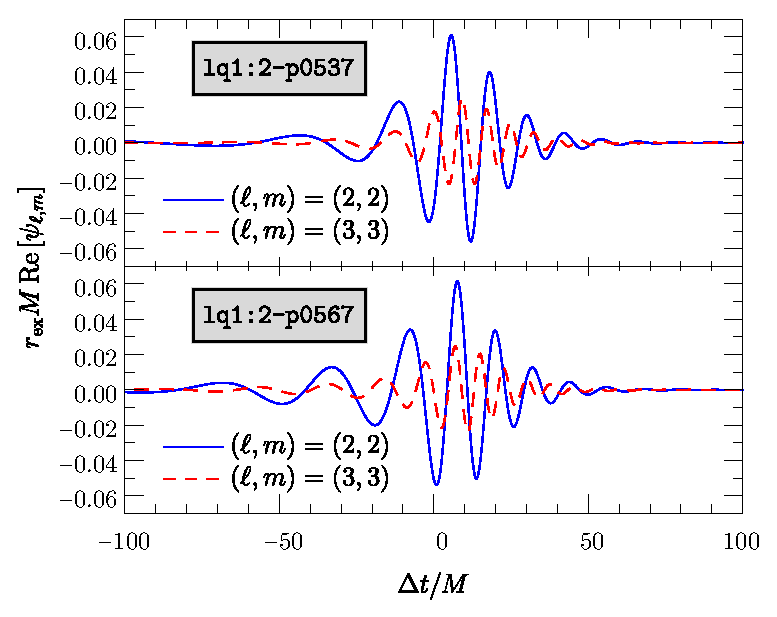
\includegraphics[width=\columnwidth]{mode-kick-extrema.eps}
			}
			\vspace{-1.5em}
			\begin{itemize}
 				\item<.-> Top: $v=128\text{ km/s}$
 				\item<.-> bottom: $v=173\text{ km/s}$
	 		\end{itemize}
		\column{0.55\textwidth}
			\begin{itemize}
				\item<.->
					Unlike for the radiated energy, the radiated momentum
					involves complex (in both senses of the word) 
					\alert{interactions} between different multipoles
					[cf. Eq.~\eqref{eq:P+rad}]
                \note[item]<.->{
                    For example the $\tl=2,\tm=-2$ term in the sum involves
                    contributions from the $(2,-2)$, $(2,1)$ and $(3,3)$
                    multipoles of $\Psi_4$.}
				\item<+->
					On the left, the $(\ell,m)=(2,2)$ and $(3,3)$, 
					modes of $\Psi_4$ are shown for two \alert{consecutive} 
					local extrema on the
					curves $v=v(p)$ for \texttt{lq1:2} ($\Delta t=0$ at common 
					AH formation).
                \note[item]<.->{
                    By consecutive extrema, we mean a minimum and a maximum
                    that are next to each other on the kick against $p$ plot.}
				\item<+->
					The modes appear to be more \alert{in phase} for the 
					bigger kick 
					and more \alert{in antiphase} for the smaller kick.
                \note[item]<.->{
                    Point out with laser pointed}
				\item<+->
					This pattern is observed for other 
					sequences/consecutive extrema.
                \note[item]<.->{
                    This is merely an observation and we don't have a good
                    understanding of this phenomenon. This warrants further
                    investigation.}
			\end{itemize}
	\end{columns}
\end{frame}

\section{Conclusion}

\begin{frame}{Summary}
    \begin{itemize}
        \item<+->
            We have evolved 274 BBH configurations with mass ratio 
            $q=2/3$, $1/2$ and $1/3$ spread across four 
            sequences with \textsc{GRChombo} and \textsc{Lean}.
    %     \item<+->
    %     	We have demonstrated that \textsc{GRChombo} is capable of 
    %     	evolving BBH inspirals with \alert{comparable accuracy} to a more 
    %     	established NR code.
        \item<+->
            For all sequences, we observe \alert{oscillations} in the kick as a 
            function of eccentricity with
            a global maximum at $e\sim0.5$. These oscillations differ
            from that of the final spin and radiated energy.
        \item<+->
            We posit that this oscillatory behaviour is due to the change in the
            \alert{infall direction} relative to the \alert{apo/periapsis}. 
        \item<+->
            We find that longer inspirals lead to bigger and 
            more frequent oscillations
        \item<+->
            We observe shifts in the \alert{phase} of subdominant 
            multipoles of $\Psi_4$ relative to the dominant $(2,2)$ mode
            between larger and smaller kicks.
    \end{itemize}
\end{frame}

\begin{frame}{Implications and future avenues}
    \begin{itemize}
        \item<+->
            Longer simulations gave us more sensitive dependence on 
            eccentricity. What about circularizing nature of GW emissions?
        \note[item]<.->{
            In certain astrophysical scenarios/environments e.g. some 3-body 
            systems, we might expect the interaction of the 3rd body to retain 
            or even increase the eccentricity of the binary and this could
            outcompete the effect of GW emissions.}
        \item<+->
            Need to investigate more quantitatively the differences in GW 
            signals.
        \note[item]<.->{
            There may be implications for parameter inference in GW 
            observations}
        \item<+->
            Use PN methods to investigate long eccentric inspirals on 
            astrophysical timescales.
        \item<+->
            Main takeaway: rich phenomenology of GWs from eccentric compact 
            binaries.
        \note[item]<.->{
            With more advanced GW detectors on the horizon promising increased
            sensitivity in certain frequency bands the need to understand 
            this phenomenology better is only going to grow.}
    \end{itemize}
\end{frame}

\section*{Any questions?}

\appendix
\begin{frame}{Convergence and comparison between 
\textsc{GRChombo} and \textsc{Lean}}
    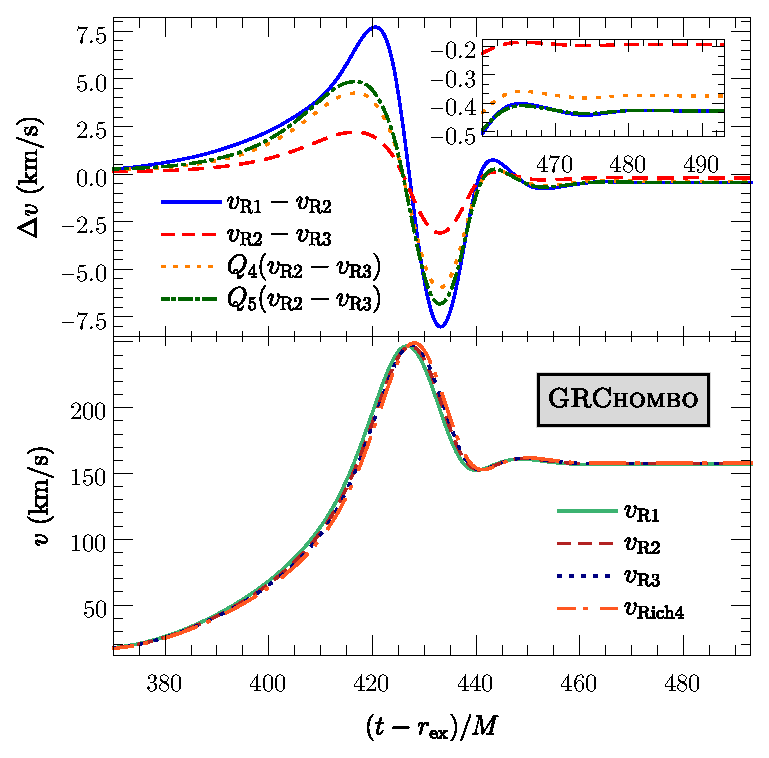
\includegraphics[width=0.45\linewidth]{grchombo-convergence5.eps}
    \hfill
    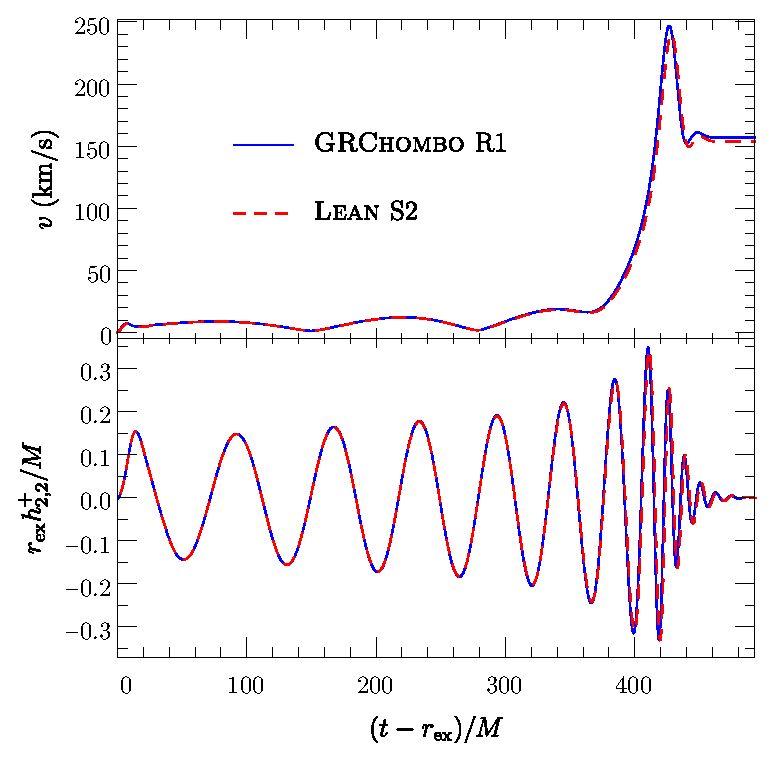
\includegraphics[width=0.45\linewidth]{grchombo-lean-comparison3.eps}
\end{frame}

\begin{frame}{CCZ4 equations}
    \footnotesize
    The Z4 equation of motion is
    \begin{equation*}
       {}^{(4)}R_{ab} + 2\nabla_{(a} Z_{b)} -
        2\kappa_1 n_{(a} Z_{b)} + \kappa_1(1 + \kappa_2)g_{ab}n_c Z^c 
        = 8\pi \left(T_{ab} - \frac{1}{2}g_{ab}T\right).
    \end{equation*}
    The CCZ4 system is then
    \begin{align*}
		\partial_t\chi &= \beta^k\partial_k\chi + \frac{2}{3}\chi(\alpha K - 
        \partial_k\beta^k),\label{eq:CCZ4-chi}\\
		\partial_t\tilde{\gamma}_{ij} &= \beta^k\partial_k\tilde{\gamma}_{ij} 
        +\tilde{\gamma}_{ki}\partial_j\beta^k + 
        \tilde{\gamma}_{kj}\partial_i\beta^k -2\alpha \tilde{A}_{ij} - 
        \frac{2}{3}\tilde{\gamma}_{ij}\partial_k\beta^k,\\
        \partial_t K &= \beta^k\partial_k K + \alpha \left(R + 
        \color{blue}2D_k Z^k\normalcolor + 
        K(K\color{blue}-2\Theta\normalcolor)\right)\color{red} - 
        3\alpha\kappa_1(1+\kappa_2)\Theta \normalcolor- 
        \gamma^{kl}D_kD_l\alpha + 4\pi\alpha (S - 3\rho),\\
		\begin{split}
			\partial_t\tilde{A}_{ij} &= \beta^k\partial_k \tilde{A}_{ij} + 
            \chi\left[-D_iD_j\alpha + \alpha(R_{ij} + \color{blue} 
            2D_{(i}Z_{j)} \normalcolor - 8\pi S_{ij}) \right]^{\mathrm{TF}} + 
            \tilde{A}_{ij} \left[\alpha(K \color{blue} - 2\Theta\normalcolor) - 
            \frac{2}{3}\partial_k\beta^k\right]
            + 2\tilde{A}_{k(i}\partial_{j)}\beta^k -\\ 
            &\qquad 2\alpha\tilde{\gamma}^{kl}\tilde{A}_{ik}\tilde{A}_{lj},
		\end{split}\\
		\begin{split}
			\partial_t\Theta &= \beta^k\partial_k\Theta + 
            \frac{1}{2}\alpha\left(R + 2D_k Z^k - \tilde{A}_{kl}\tilde{A}^{kl} 
            + \frac{2}{3}K^2 \color{blue}- 2\Theta K\normalcolor\right)
			\color{red} - \kappa_1\alpha\Theta(2 + \kappa_2)\color{blue}- 
            Z^k\partial_k\alpha\normalcolor - 8\pi \alpha \rho,
		\end{split}\\
		\begin{split}
			\partial_t\color{blue}\hat{\Gamma}^i\normalcolor &= 
            \beta^k\partial_k\color{blue}\hat{\Gamma}^i\normalcolor + 
            \frac{2}{3}\left[\partial_k\beta^k\left(\tilde{\Gamma}^i 
            \color{teal} + 
            2\kappa_3\frac{Z^i}{\chi}\normalcolor\right)\color{blue} - 2\alpha 
            K\frac{Z^i}{\chi}\normalcolor\right]  -\color{red} 
            2\alpha\kappa_1\frac{Z^i}{\chi}\normalcolor
			+\color{blue} 2\tilde{\gamma}^{ij}(\alpha\partial_j\Theta - 
            \Theta\partial_j\alpha)- 2\tilde{A}^{ij}\partial_j\alpha \\
            &\qquad\normalcolor
            - \alpha\left[\frac{4}{3}\tilde{\gamma}^{ij}\partial_jK + 
            3\tilde{A}^{ij}\frac{\partial_j\chi}{\chi}\right]
            - \left(\tilde{\Gamma}^j \color{teal}+ 
            2\kappa_3\frac{Z^j}{\chi}\normalcolor\right)\partial_j\beta^i + 
            2\alpha\tilde{\Gamma}^i_{jk}\tilde{A}^{jk} + 
            \tilde{\gamma}^{jk}\partial_j\partial_k\beta^i + 
            \frac{1}{3}\tilde{\gamma}^{ij}\partial_k\partial_j\beta^k - 16\pi 
            \alpha\tilde{\gamma}^{ij}S_j.
		\end{split}
	\end{align*}
\end{frame}

\begin{frame}{Moving Puncture Gauge}
    The equations of motion for the lapse and shift in the moving puncture
    gauge are
    \begin{align*}
        \partial_t\alpha &= \beta^k\partial_k\alpha -2\alpha(K-2\Theta),\\
        \partial_t\beta^i &= \beta^k\partial_k\beta^i + \frac{3}{4} B^i, \\
        \partial_tB^i &= \beta^k\partial_kB^i + (\partial_t 
        - \beta^k\partial_k)\hat{\Gamma}^i  - \eta B^i.
    \end{align*}
\end{frame}

\end{document}


